%! Author = sutingchen
%! Date = 2023/10/18

\titledquestion{Generate a binary tree}

\begin{parts}
    \part[4] Given the in-order and pre-order traversal of a binary tree T are \textbf{ECFBDGA} and \textbf{ABCEFDG} respectively.\\
    Draw the tree T.\\
    \begin{solution}
        $$ $$
        \centering
        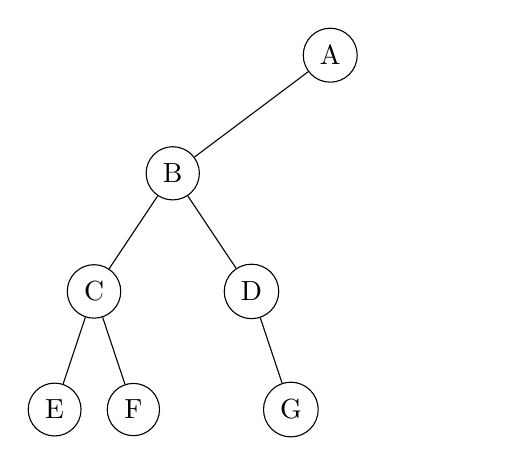
\begin{tikzpicture}[level distance=1.5cm,
                level 1/.style={sibling distance=4cm},
                level 2/.style={sibling distance=2cm},
                level 3/.style={sibling distance=1cm},
                every node/.style = {draw, circle}
            ]
            \node {A}
            child { node {B}
                    child { node {C}
                            child { node {E} }
                            child { node {F} }
                        }
                    child { node {D}
                            child { edge from parent[draw=none] }
                            child { node {G} }
                        }
                }
            child { edge from parent[draw=none]};
        \end{tikzpicture}
        $$ $$
    \end{solution}
    % \vspace{2cm}
    \part[4] Given the in-order and post-order traversal of a binary tree T are \textbf{EBDAHCGF} and \textbf{EDBHFGCA} respectively.\\
    Draw the tree T.\\
    \begin{solution}
        $$ $$
        \centering
        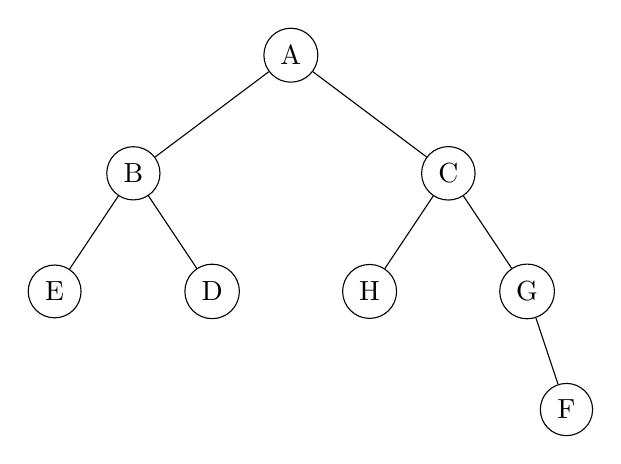
\begin{tikzpicture}[level distance=1.5cm,
                level 1/.style={sibling distance=4cm},
                level 2/.style={sibling distance=2cm},
                level 3/.style={sibling distance=1cm},
                every node/.style = {draw, circle}
            ]
            \node {A}
            child { node {B}
                    child { node {E} }
                    child { node {D} }
                }
            child { node {C}
                    child { node {H} }
                    child { node {G}
                            child { edge from parent[draw=none] }
                            child { node {F} } }
                };
        \end{tikzpicture}
        $$ $$
    \end{solution}
    % \vspace{2cm}
    \pagebreak
    \part[2] Given the pre-order and post-order traversal of a binary tree T, can you decide the tree T? If yes, please describe an algorithm to construct T; if no, please provide a counterexample.\\
    \begin{solution}\\
        No

        $$
        \begin{tikzpicture}[level distance=1.5cm,
                level 1/.style={sibling distance=4cm},
                level 2/.style={sibling distance=2cm},
                level 3/.style={sibling distance=1cm},
                every node/.style = {draw, circle}
            ]
            \node {A}
            child { node {B} }
            child { edge from parent[draw=none] };
        \end{tikzpicture}
        \text{and}
        \begin{tikzpicture}[level distance=1.5cm,
                level 1/.style={sibling distance=4cm},
                level 2/.style={sibling distance=2cm},
                level 3/.style={sibling distance=1cm},
                every node/.style = {draw, circle}
            ]
            \node {A}
            child { edge from parent[draw=none] }
            child { node {B} };
        \end{tikzpicture}
        $$

        \medskip

        are different trees, but they have same post, in, pre ordering.
    \end{solution}
\end{parts}